\documentclass{beamer}
\usepackage[utf8]{inputenc}
\usepackage{xeCJK} 
\usepackage[T1]{fontenc}
\usepackage{mathabx}
\usepackage{amsmath} 
\usepackage{mathpazo}
\usepackage{bibentry}
\usepackage{tikz}
\usepackage{caption}
\usepackage{graphicx, subfig}

\usetikzlibrary{scopes}
\def\iangle{35} % Angle of the inclined plane
\def\down{-90}
\def\arcr{0.5cm} % Radius of the arc used to indicate angles

\usetheme{Boadilla}
\usecolortheme{wolverine}
\useoutertheme{miniframes}

\title{VP160 Final Exam Review Class}
% \subtitle{Non-inertial FoR}
\author{Zeyi Ren}
\institute{UM-SJTU Joint Institute}

\begin{document}

\maketitle

\frame{\tableofcontents}

\section{Lagrangian Mechanics}
\begin{frame}
  \begin{block}{Generalized coordinates}
    Any coordinates describing motions.
  \end{block}
  e.g.
  \begin{figure}[H]
  \centering
  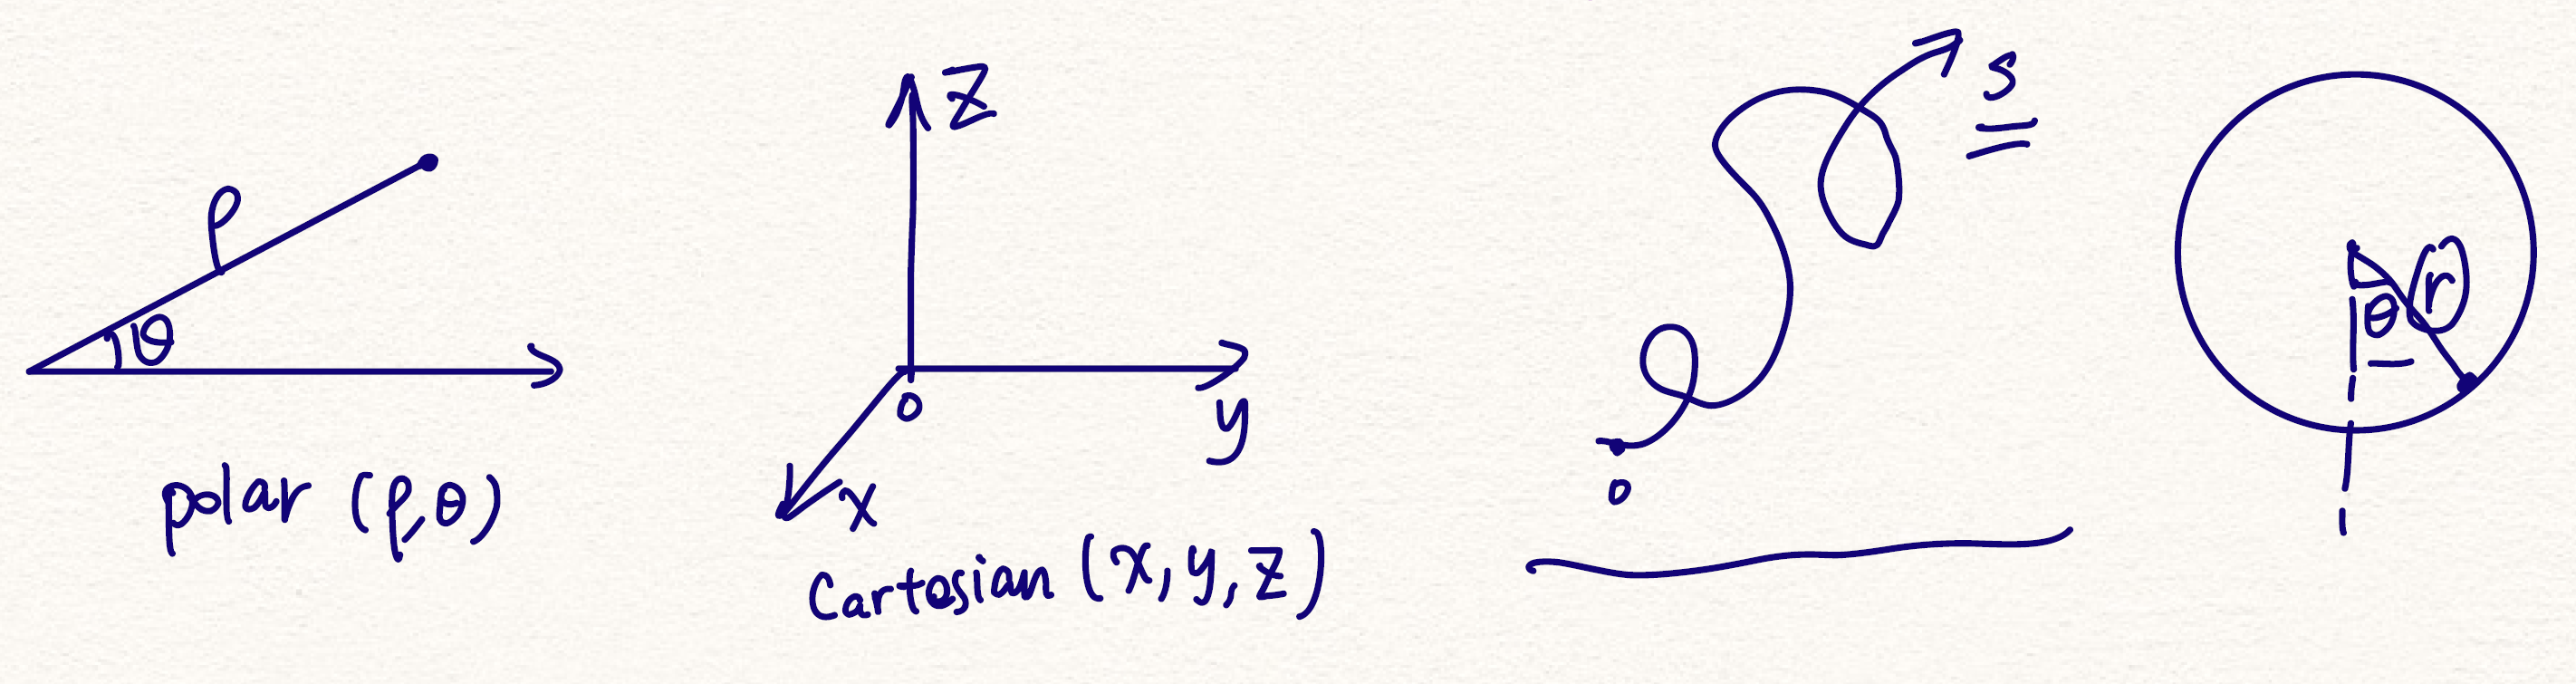
\includegraphics[width= 0.6\linewidth, angle =0]{example1.png}
  % \caption{.}
  \label{fig:1}
  \end{figure}
  \begin{block}{Degree of freedom (f)}
    The minimum number of independent generalized coordinates needed to describe the system's motions.
  \end{block}
  $$
  f = 3N - m
  $$
  where $N$ is the number of particles, and $m$ is the number of constraints (equations that relate unknowns).
\end{frame}

\begin{frame}
  \begin{block}{Hamilton's Principle (math detail don't required)}
    \begin{center}
    Real path $\Longleftrightarrow$ $\delta S = 0$\\ ($\delta$: variational differential, $S$ is a functional: a function that maps functions into numbers.)
    \end{center}
  \end{block}
  \begin{block}{Euler-Lagrange Equation}
    For $i = 1, 2,...,f$:
    $$
    \frac{d}{dt}(\frac{\partial L}{\partial \dot{q_i}})-\frac{\partial L}{\partial q_i} = 0
    $$
  \end{block}
\end{frame}

\begin{frame}
\textcolor{blue}{Exercise 1}

\begin{figure}[htbp]
\centering
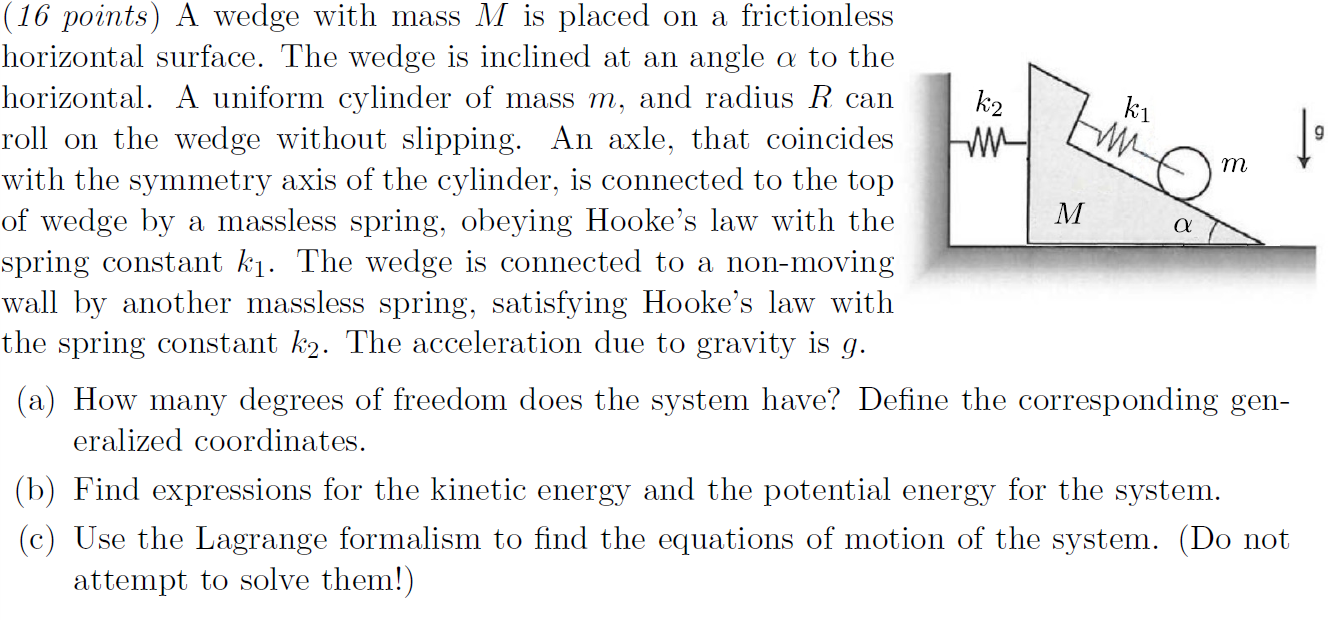
\includegraphics[width=1 \linewidth, angle =0]{ex1.png}
%\caption{.}
\label{fig:2}
\end{figure}
\end{frame}

\section{Momentum}
\begin{frame}
  \begin{block}{Definition}
    $$\vec{p} = m\vec{v}$$
  \end{block}
  \begin{block}{Rewrite Newton's second law}
    $$\vec{F}=\frac{d\vec{p}}{dt}$$ (when $m$ is not varying, $F = m\frac{d\vec{v}}{dt}=m\vec{a}$)
  \end{block}
  \begin{block}{Impulse Theorem}
    $$\vec{p_2}-\vec{p_1}=\int_{t_1}^{t_2}\vec{F}dt$$
  \end{block}
  \begin{itemize}
    \item If $\vec{F_{ext}} = 0$, for a system, $\Delta\vec{p} = 0 \Leftrightarrow \vec{p} = \text{Const}$ (Conservation of momentum)
  \end{itemize}
\end{frame}

\begin{frame}{Collision}
  \begin{itemize}
    \item Non-central Collision (e.g. explosion)
    $$\vec{p_{before}} = \vec{p_{after}}$$
    \item Central Collision
    \begin{itemize}
      \item Elastic
      \begin{itemize}
        \item $e = (\vec{v_2}'-\vec{v_1}')/(\vec{v_1}-\vec{v_2})= 1$ (seperating speed / approaching speed)
        \item Conservation of energy
      \end{itemize}
      \item Inelastic
      \begin{itemize}
        \item $e < 1$
        \item Energy loss
      \end{itemize}
      \item Completely Inelastic
      \begin{itemize}
        \item $e = 0$
        \item stick to each other
      \end{itemize}
    \end{itemize}
  \end{itemize}
\end{frame}

\begin{frame}
\textcolor{blue}{Exercise 2}

Assume $m_1$, $m_2$, $m_3$, $k$ is known. Release $m_1$, the collision between $m_1$ and $m_2$ is completely inelastic. Find $h$ so that $m_3$
can just leave the ground.
\begin{figure}[htbp]
\centering
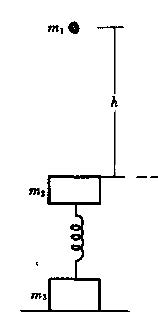
\includegraphics[width=0.2 \linewidth, angle =0]{ex5.png}
% \caption{.}
\label{fig:3}
\end{figure}
\textcolor{blue}{Answer: $\frac{(m_1+m_2)[(m_1+m_2+m_3)^2-m_2^2]}{2km_1^2}$}
\end{frame}

\begin{frame}
  \begin{block}{Center of Mass}
    $$\vec{r_C} = \frac{\sum m_i\vec{r_i}}{\sum m_i}$$ 
    $$ \vec{r_C} = \frac{\int_{}^{} \vec{r_i} dm}{\int_{}^{} dm}$$
  \end{block}
  \begin{block}{Pappus Law (Another way to derive center of mass)}
    First Theorem (for object with linear mass density): $$S = 2\pi sx\text{ ($s$ the curve length)}$$ 
    Second Theorem (for plane): $$V = 2\pi Ax\text{ ($A$ the plane area)}$$ 
  \end{block}
  where $x$ is the distance from the reference axis and the center of mass.
\end{frame}

\begin{frame}
  \begin{figure}[H]
    \centering
    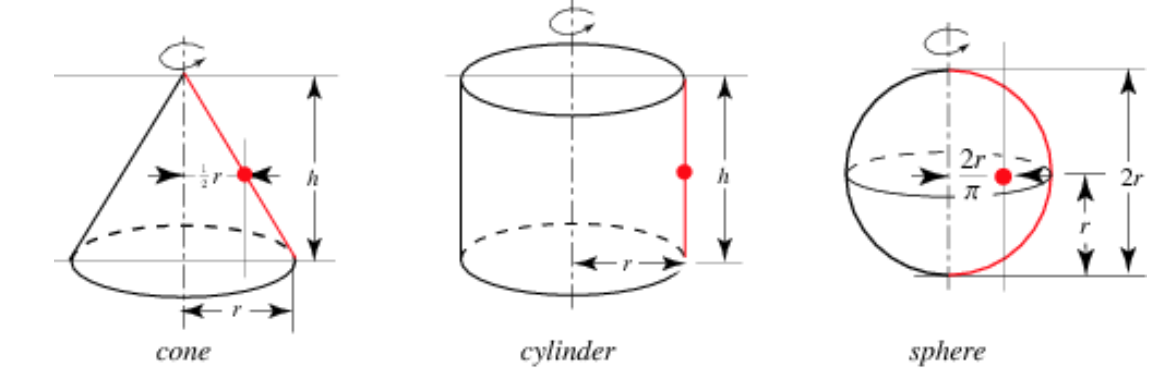
\includegraphics[width=0.6 \linewidth, angle =0]{example3.png}
    % \caption{.}
    \label{fig:6}
    \end{figure}
    \begin{figure}[htbp]
    \centering
    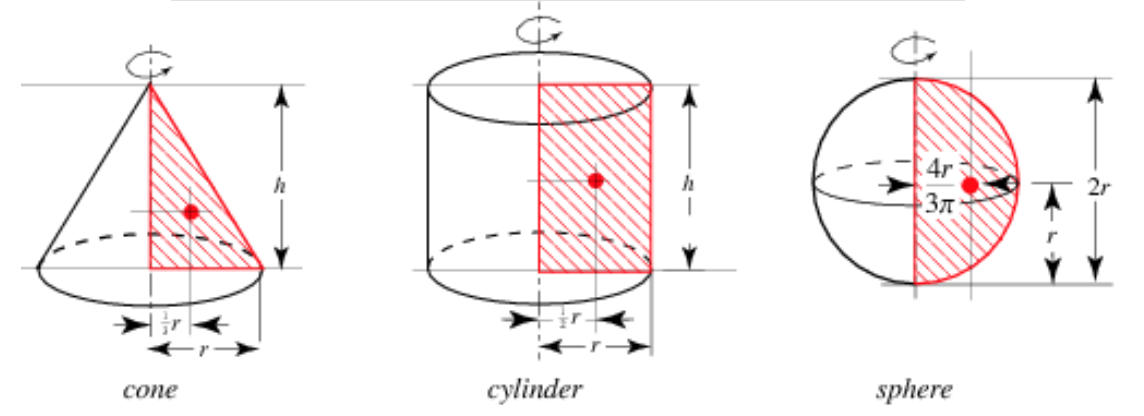
\includegraphics[width=0.6 \linewidth, angle =0]{example2.png}
    % \caption{.}
    \label{fig:7}
    \end{figure}\pause
    \begin{itemize}
      \item An important fact (for any system (total mass = constant), e.g. rigid body): $$\vec{F_{ext}} =\dot{\vec{p}}= M\dot{\vec{v_c}}$$
    \end{itemize}
\end{frame}
\begin{frame}{Mass Variation Problem}
  \begin{block}{Rocket Propulsion}
    $$mv + Fdt = (m+dm)(v+dv)-udm$$
    $$m\frac{dv}{dt} = (u-v)\frac{dm}{dt}+ F$$
    \end{block}
    \textcolor{blue}{Reminder:}
    What FoR are we looking at?\\
    Some string problems?\\
    \textcolor{blue}{Tips:}\\
    \begin{itemize}
      \item infinitesimal methods
      \item write out $F = \frac{dp}{dt}$, find out what is $p$, e.g. $p = \lambda v x$.
    \end{itemize}
\end{frame}

\begin{frame}
\textcolor{blue}{Exercise 3}

An unpowered aircraft of mass $m$ and initial velocity $v_0$ is moving in space dust. During the movement, the aircraft will absorb the dust. The mass absorbed onto the craft is proportional to the distance $s$ it traveled, the coefficient is $\alpha$, $m_{absorb} = \alpha s$.\\
i) Determine the total distance traveled by the aircraft before stopping.\\
ii) Determine the relationship between aircraft movement speed and time.\\
~\\
\textcolor{blue}{Answer: i) $s\rightarrow \infty$ ii) $v = \frac{v_0}{\sqrt{1+\frac{2\alpha v_0}{m_0}t}}$}
\end{frame}

\begin{frame}
\textcolor{blue}{Exercise 4}

A uniform soft rope of length $l$ and mass linear density $\lambda$ is hung on the ceiling. At the beginning, both ends $A$ and $B$ are hung on the fixed point together, then B begins to fall freely from the suspension point. When the drop height of the B end is $x < l$, try to find the magnitude of the tensile force at the suspension point.

\begin{figure}[htbp]
\centering
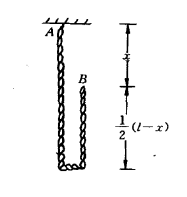
\includegraphics[width=0.3 \linewidth, angle =0]{string.png}
%\caption{.}
\label{fig:100}
\end{figure}
\textcolor{blue}{Answer: $T = \frac{1}{2}(l+3x)\lambda g$}
\end{frame}

\section{Equilibrium \& Elasticity}
\begin{frame}
  \begin{block}{Equilibrium}
    %The sum of all the external forces is equal to zero
    $$\vec{F_{ext}} = 0$$
    %The sum of all torques of external forces about any point is equal to zero
    $$\vec{\tau_{ext}} = 0$$
  \end{block}
  \begin{itemize}
    \item The sum of all the external forces is equal to zero
    \item The sum of all torques of external forces about any point is equal to zero
  \end{itemize}
  $$\Rightarrow \text{If the object is initially at rest, then it will remain at rest.}$$
\end{frame}

\begin{frame}
  \begin{block}{Center of Gravity}
    A point from which the weight of a body or system may be considered to act. In uniform gravity it is the same as the center of mass.
  \end{block}
  \begin{itemize}
    \item For translational motion: $$\vec{G} = M\vec{a_c}$$
    \item For rotation: $$\vec{\tau_{tot}} = \sum \vec{r_i}\times \vec{G_i}$$
    If in a uniform gravitaional field (mostly):
    $$\vec{\tau_{tot}}= \sum m_i\vec{r_i}\times \vec{g} = M\frac{\sum m_i\vec{r_i}}{\sum m_i}\times \vec{g} = M\vec{r_c}\times \vec{g} = \vec{r_c}\times \vec{G}$$
  \end{itemize}
\end{frame}

\begin{frame}{Methods for Solving Statics}
  \textcolor{blue}{Review RC\_wk10\_withnotes for detail!}
  \begin{enumerate}
    \item Equilibrium equations.
    \begin{itemize}
      \item Translational motion: Force
      \item Rotation: Torque
    \end{itemize}
    \item Infinitesimal methods
    \item Derivation of energy
    \begin{itemize}
      \item $\frac{\partial U}{\partial q_i} = 0$, the system potential energy reaches an local minimum.
      \item useful for low degree of freedom system.
    \end{itemize}
  \end{enumerate}
\end{frame}

\begin{frame}
  \begin{block}{Stress}
    Stress is the force per unit area.
  \end{block}
  \begin{block}{Strain}
    Strain is the fractional deformation due to the stress.
  \end{block}
  $$\text{elastic modulus } = \frac{\text{stress}}{\text{strain}}$$
\end{frame}

\begin{frame}
  \begin{block}{Young's modulus: tensile stress divided by tensile strain}
    $$Y = \frac{\frac{F\bot }{A}}{\frac{\Delta l}{L}}$$
  \end{block}
  \begin{figure}[htbp]
  \centering
  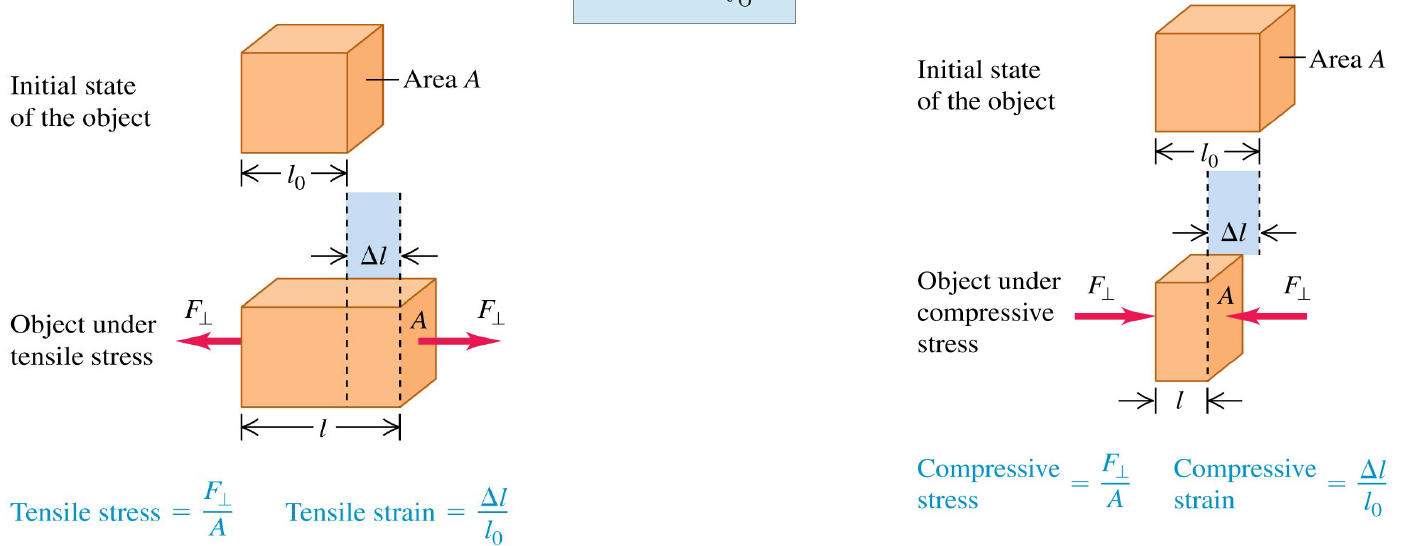
\includegraphics[width=1 \linewidth, angle =0]{y's.png}
  %\caption{.}
  \label{fig:y's}
  \end{figure}
\end{frame}

\begin{frame}
  \begin{block}{Bulk's modulus: bulk stress divided by bulk strain}
    $$B=-\frac{\Delta p}{\frac{\Delta v}{V}}$$
  \end{block}
  \begin{figure}[htbp]
  \centering
  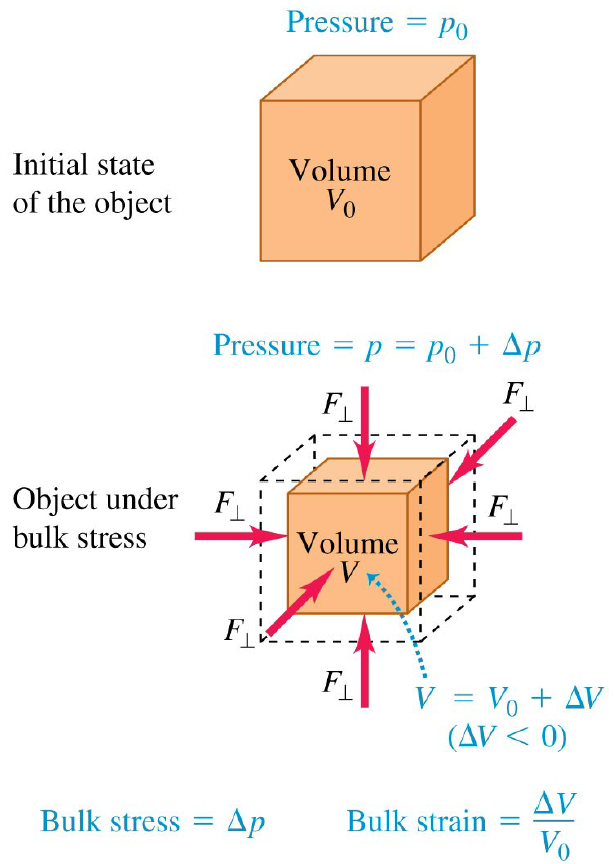
\includegraphics[width=0.4 \linewidth, angle =0]{b's.png}
  %\caption{.}
  \label{fig:b's}
  \end{figure}
\end{frame}

\begin{frame}
  \begin{block}{Shear modulus: shear stress divided by shear strain}
    $$S=\frac{\frac{F_{\|}}{A}}{\frac{X}{h}}$$
  \end{block}
  \begin{figure}[htbp]
  \centering
  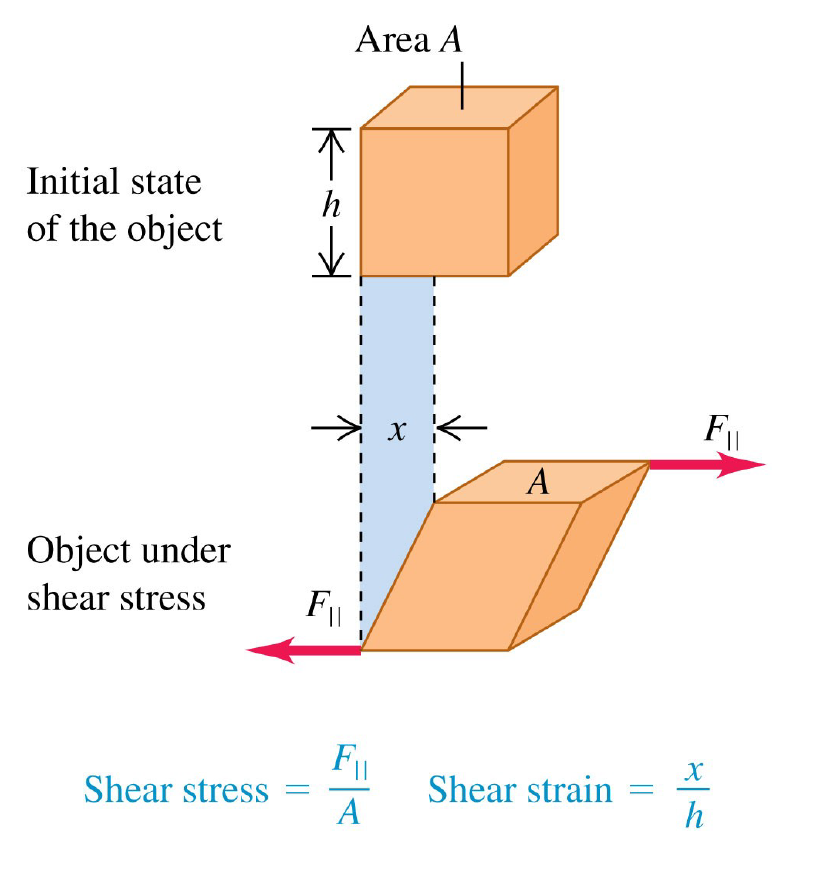
\includegraphics[width=0.4 \linewidth, angle =0]{s's.png}
  %\caption{.}
  \label{fig:s's}
  \end{figure} 
\end{frame}

\section{Fluid Dynamics}
\begin{frame}
  \begin{block}{Pressure at a Depth}
    $$dp = -\rho g dy$$
    $$p = p_0 + \rho gh$$
  \end{block}
  \begin{block}{Pascal's Law}
    Pressure applied to an enclosed incompressible fluid is transmitted
undiminished to every portion of the liquid and the walls of the container.
  \end{block}
  \begin{block}{Guage Pressure vs. Absolute Pressure}
    Absolute: $p = p_{atm}+p_{gauge}$\\
    Gauge: $p_{gauge} = p - p_{atm}$ 
  \end{block}
  $1atm = 101325Pa = 760mmHg$\\  
  Every $10m$ depth of water adds to a pressure of $1atm$.
\end{frame}
\begin{frame}
  Surface Tension:
  \begin{figure}[htbp]
  \centering
  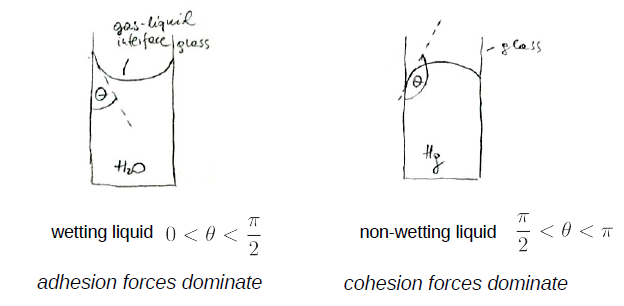
\includegraphics[width=0.9 \linewidth, angle =0]{surface.png}
  %\caption{.}
  \label{fig:surface}
  \end{figure}
\end{frame}

\begin{frame}
  \begin{block}{Continuity Equation}
    $$A_1 v_1 = A_2 v_2$$
  \end{block}
  \begin{block}{Bernoulli's Equation}
    \begin{centering}
    $\delta W = dK + dU$\\
    $(p_1-p_2)dV = \frac{1}{2}\rho (v_2^2 - v_1^2)dV + \rho g(y_2-y_1)dV$\\
    $$\Rightarrow p + \frac{1}{2}\rho v^2 + \rho gy = \text{const}$$
    \end{centering}
  \end{block}
\end{frame}

\section{Gravitaion}
\begin{frame}
  \begin{block}{Basic formulas}
    Force: $$\vec{F}= -\frac{GMm}{r^3}\vec{r}$$
    Gravitational Potential Energy:
    $$U = -\frac{GMm}{r} + C$$
    ($C$ depends on the choice of zero potential. Treat $r = \infty$ as the zero potential, then $C = 0$)
  \end{block}
\end{frame}

\begin{frame}
  \begin{block}{Kepler's Laws}
    \begin{enumerate}
      \item Each planet moves in an elliptical orbit with the Sun at one
      of the focal points.
      \item The line from the Sun to a given planet sweeps out equal
      areas in equal times.
      \item $T^2/a^3$ is a constant ($=4\pi^2/GM$ if $M>>m$)
    \end{enumerate}
  \end{block}
  \textcolor{blue}{Comment:}\\
  \begin{enumerate}
    \item Law 1: hyperbolic curve: $U+K<0$ ellipse; $U+K=0$ parabola; $U+K>0$ hyperbola.
    \item Law 2: The result of the conservation of angular momentum, or to say, aerial velocity = constant.
    \item $a$ is the semi-major axis of the ellipse(半长轴).
  \end{enumerate}
\end{frame}
\begin{frame}
  \textcolor{blue}{Tips on solving satellite motion problems:}\\
  Use Conservation of Energy and Conservation of Angular Momentum!\\
  E = const: $$\frac{1}{2}mv_1^2 + (-\frac{GMm}{r_1^2}) = \frac{1}{2}mv_2^2 + (-\frac{GMm}{r_2^2})$$
  L = const: $$mv_1r_1 = mv_2r_2$$ 
\end{frame}
\begin{frame}
\textcolor{blue}{Exercise 5}

Consider a hollow thick spherical shell with a mass density of $\rho$ as showed in the figure, calculate the gravitational force exerted on the three particles $m_1, m_2, m_3$ (only consider the force between the spherical shell and the particle)
\begin{figure}[htbp]
\centering
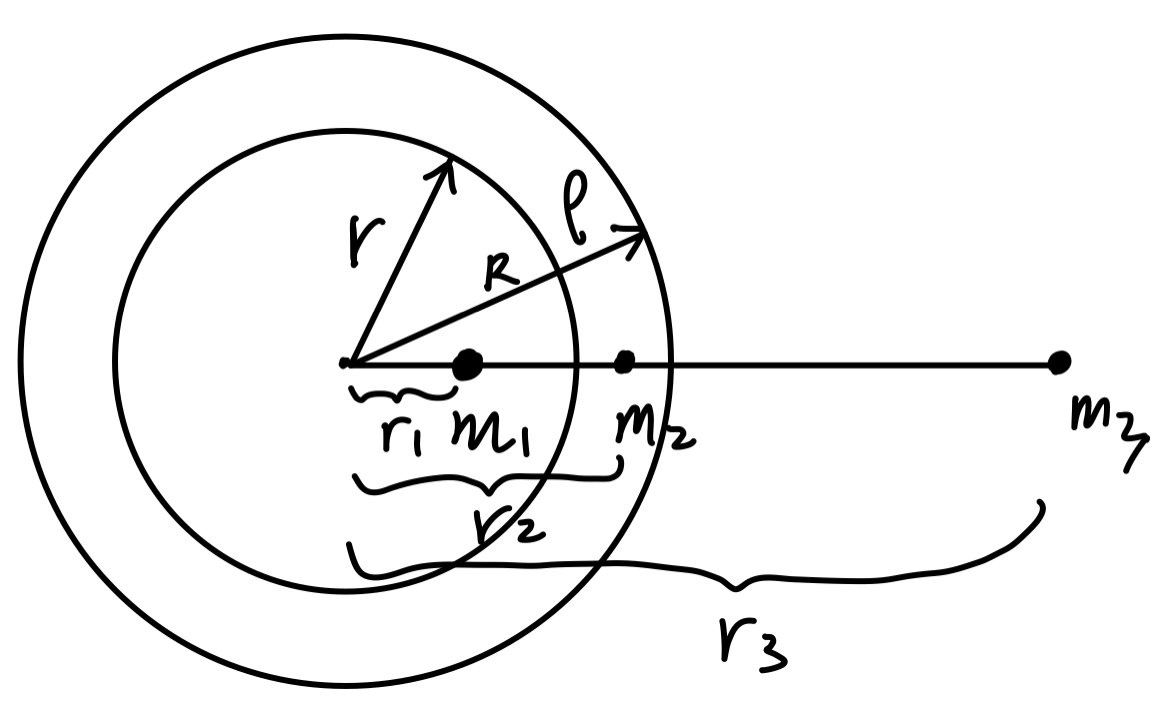
\includegraphics[width=0.4 \linewidth, angle =0]{sph.png}
%\caption{.}
\label{fig:sph}
\end{figure}
How to calculate the gravitaional filed caused by a spherically symmetric mass distribution (what is spherically symmetric distribution?)\\
\textcolor{blue}{recall hw12 p6 Gauss Law for gravitational force: $\int\int_{\sum}\mathbf{E_G}\hat{n}dS = -4\pi GM_{\sum}$}

%\begin{figure}[htbp]
%\centering
%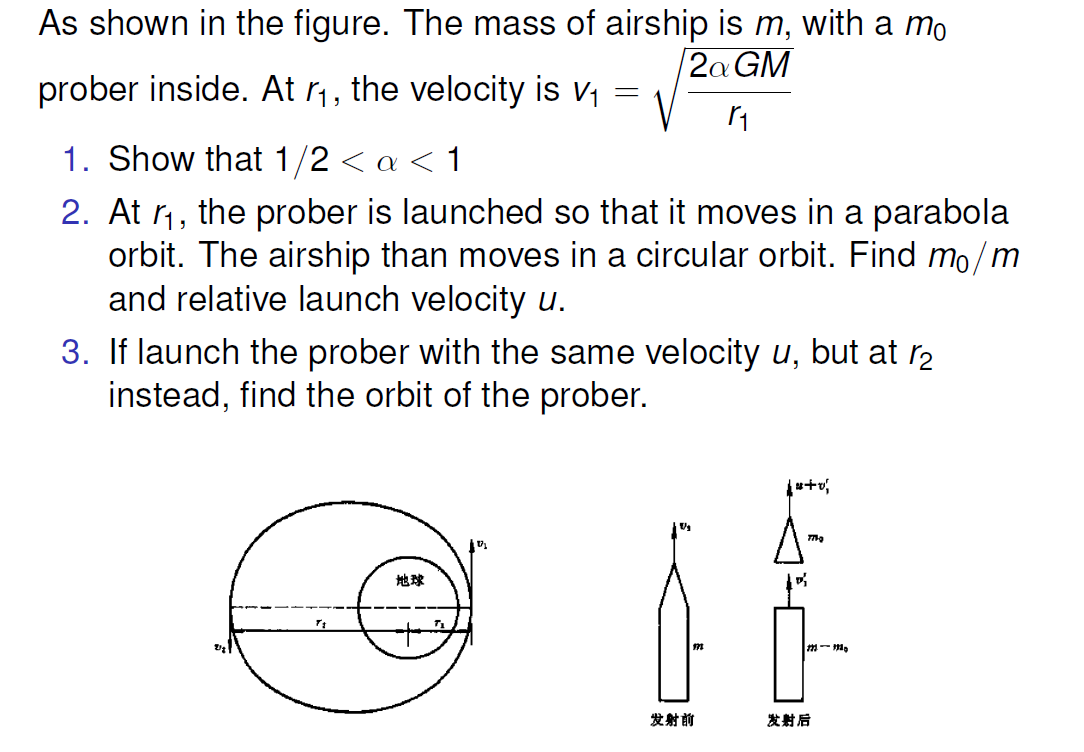
\includegraphics[width=0.92 \linewidth, angle =0]{ex_gravitation.png}
%%\caption{.}
%\label{fig:ex_gravitation}
%\end{figure}
%\end{frame}
%\begin{frame}
%  \textcolor{blue}{Answer: 2.$m/m_0 = \frac{\sqrt{2\alpha}-1}{\sqrt{2}-1}$, 3. $\alpha_0 = \sqrt{2}-\frac{1}{2}, \alpha < \alpha_0\text{ ellipse}, \alpha = \alpha_0\text{ parabola}, \alpha > \alpha_0\text{ hyperbola}$.}
\end{frame}
\begin{frame}
  \begin{center}
  \LARGE{GOOD LUCK!}
  \end{center}
\end{frame}
\end{document}



